\documentclass[tikz,border=10pt]{standalone}
\usepackage{tikz}
\usepackage{xcolor}
\usetikzlibrary{positioning,fit,calc}

% 定义颜色
\definecolor{lightblue1}{RGB}{200,220,255}
\definecolor{lightblue2}{RGB}{150,190,255}
\definecolor{lightblue3}{RGB}{100,160,255}
\definecolor{lightgreen1}{RGB}{200,255,200}
\definecolor{lightgreen2}{RGB}{150,255,150}
\definecolor{lightyellow1}{RGB}{255,255,200}
\definecolor{lightyellow2}{RGB}{255,255,150}
\definecolor{lightpink1}{RGB}{255,200,200}
\definecolor{lightpink2}{RGB}{255,150,150}
\definecolor{lightorange1}{RGB}{255,220,150}
\definecolor{lightorange2}{RGB}{255,180,100}
\definecolor{lightpurple1}{RGB}{220,200,255}
\definecolor{lightbrown}{RGB}{180,120,80}
\definecolor{lightcyan}{RGB}{150,255,255}

\begin{document}
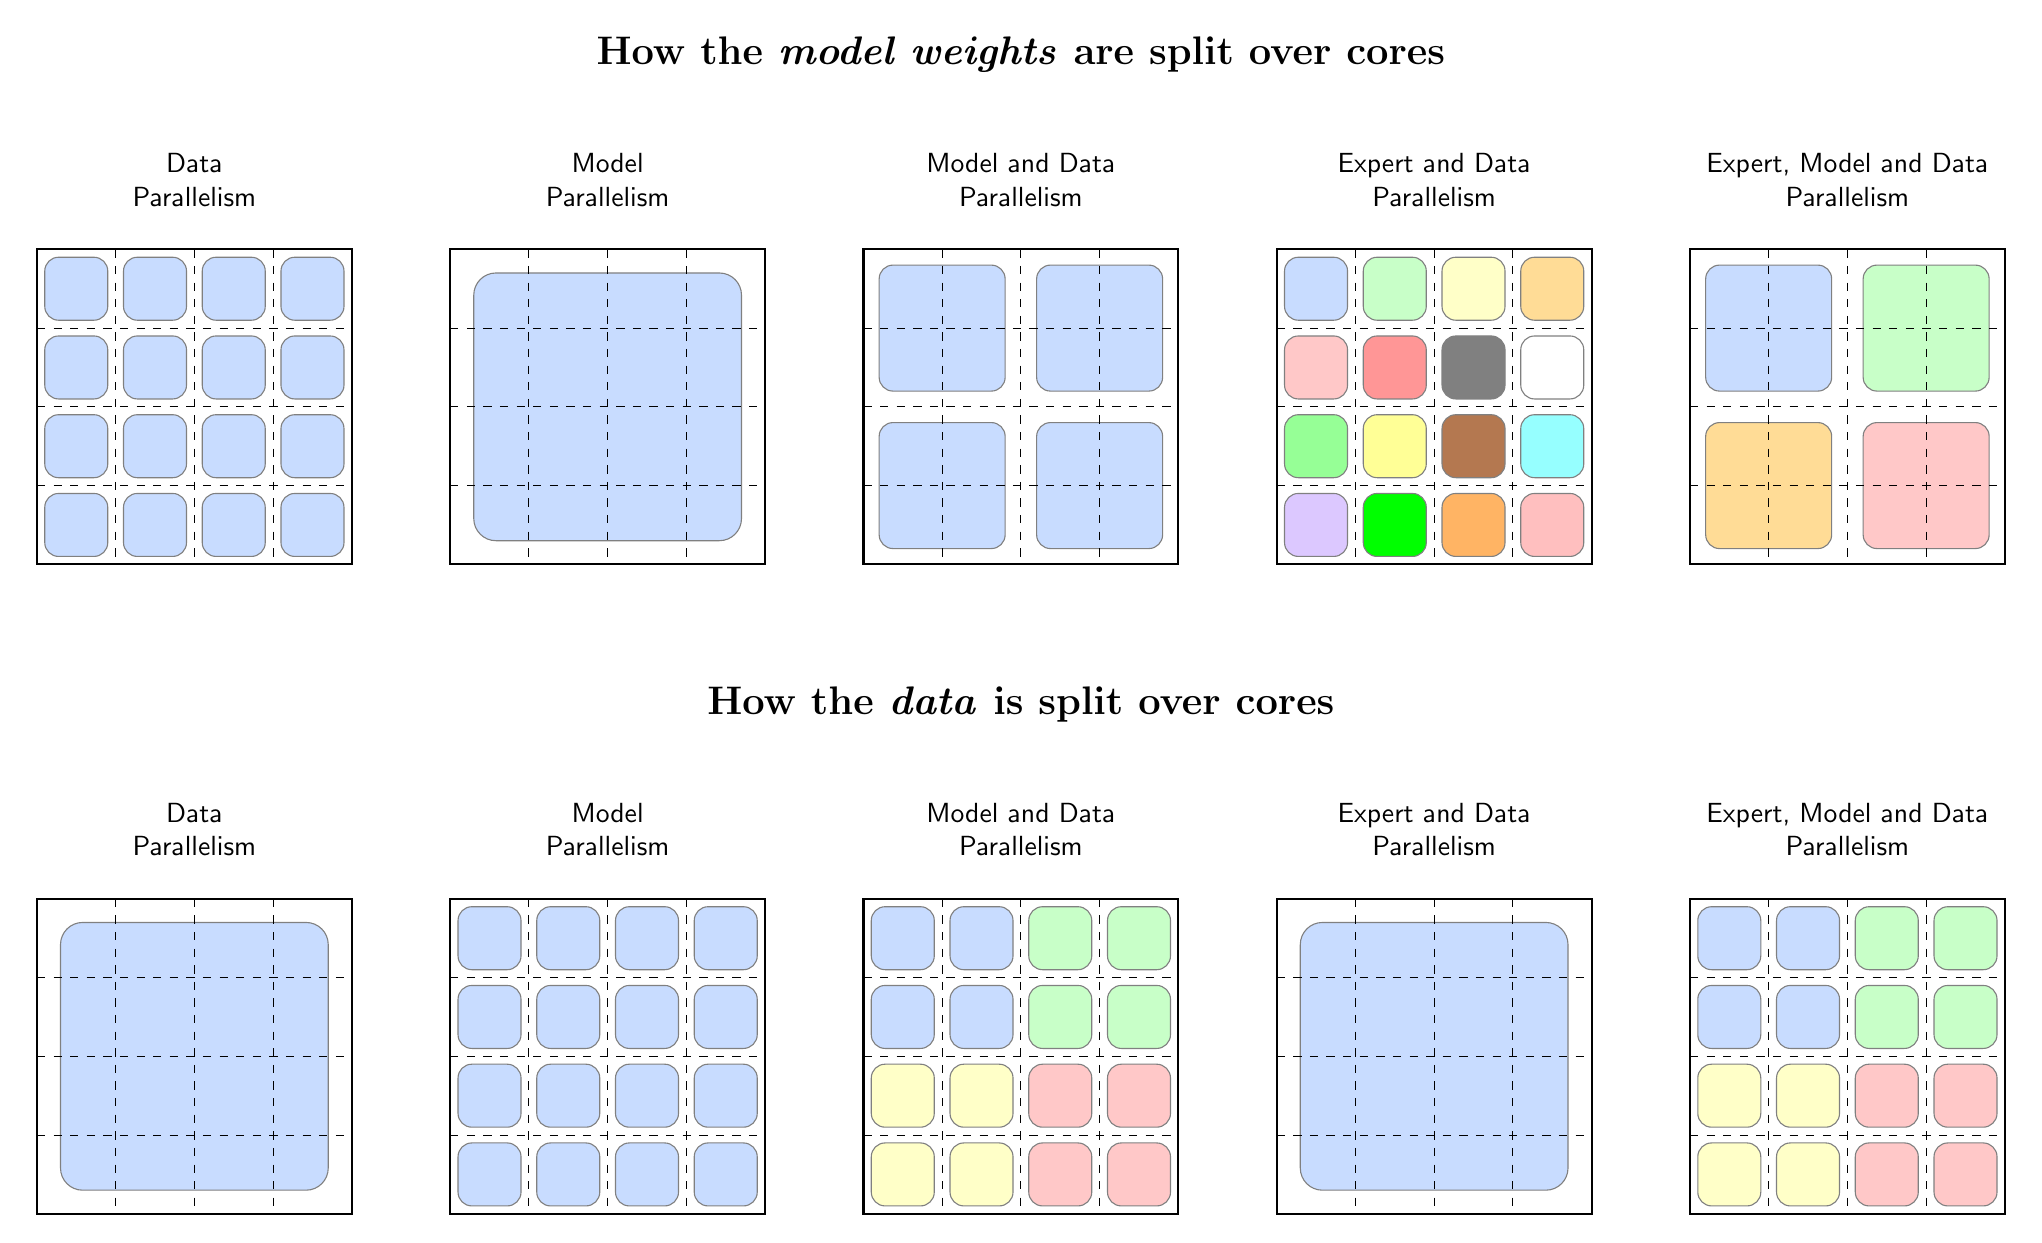
\begin{tikzpicture}[
    cell/.style={draw=black!50, minimum width=0.8cm, minimum height=0.8cm, inner sep=0pt, rounded corners=5pt},
    title/.style={font=\sffamily\Large\bfseries, anchor=center},
    subtitle/.style={font=\sffamily\normalsize, text centered, anchor=center, text width=4cm},
    diagram/.style={anchor=center},
    node distance=1.5cm
]

% 创建第一行的图表容器节点
\node[diagram] (data_par_container) {};
\node[diagram, right=5 of data_par_container] (model_par_container) {};
\node[diagram, right=5 of model_par_container] (model_data_par_container) {};
\node[diagram, right=5 of model_data_par_container] (expert_data_par_container) {};
\node[diagram, right=5 of expert_data_par_container] (expert_model_data_par_container) {};

% 第一行标题
\node[subtitle, above=0.3cm of data_par_container] {Data\\Parallelism};
\node[subtitle, above=0.3cm of model_par_container] {Model\\Parallelism};
\node[subtitle, above=0.3cm of model_data_par_container] {Model and Data\\Parallelism};
\node[subtitle, above=0.3cm of expert_data_par_container] {Expert and Data\\Parallelism};
\node[subtitle, above=0.3cm of expert_model_data_par_container] {Expert, Model and Data\\Parallelism};

% 上半部分标题
\node[title, above=2cm of model_data_par_container] (main_title1) {\rmfamily How the \textit{model weights} are split over cores};

% 第一行 - Data Parallelism
\begin{scope}[shift={($(data_par_container)-(1.5,0.5)$)}]
    \foreach \i in {0,1,2,3} {
        \foreach \j in {0,1,2,3} {
            \node[cell, fill=lightblue1] at (\i*1, -\j*1) {};
        }
    }
    \foreach \i in {0,1,2} {
        \draw[dashed] (\i+0.5, 0.5) -- (\i+0.5, -3.5);
    }
    \foreach \j in {0,1,2} {
        \draw[dashed] (-0.5, -\j-0.5) -- (3.5, -\j-0.5);
    }
    \draw[thick] (-0.5, 0.5) rectangle (3.5, -3.5);
\end{scope}

% 第二个 - Model Parallelism  
\begin{scope}[shift={($(model_par_container)-(1.5,0.5)$)}]
    \draw[fill=lightblue1, draw=black!50, rounded corners=8pt] (-0.2, 0.2) rectangle (3.2, -3.2);
    \foreach \i in {0,1,2} {
        \draw[dashed] (\i+0.5, 0.5) -- (\i+0.5, -3.5);
    }
    \foreach \j in {0,1,2} {
        \draw[dashed] (-0.5, -\j-0.5) -- (3.5, -\j-0.5);
    }
    \draw[thick] (-0.5, 0.5) rectangle (3.5, -3.5);
\end{scope}

% 第三个 - Model and Data Parallelism
\begin{scope}[shift={($(model_data_par_container)-(1.5,0.5)$)}]
    \foreach \i in {0,1} {
        \foreach \j in {0,1} {
            \node[cell, fill=lightblue1, minimum width=1.6cm, minimum height=1.6cm, rounded corners=5pt] at (\i*2+0.5, -\j*2-0.5) {};
        }
    }
    \foreach \i in {0,1,2} {
        \draw[dashed] (\i+0.5, 0.5) -- (\i+0.5, -3.5);
    }
    \foreach \j in {0,1,2} {
        \draw[dashed] (-0.5, -\j-0.5) -- (3.5, -\j-0.5);
    }
    \draw[thick] (-0.5, 0.5) rectangle (3.5, -3.5);
\end{scope}

% 第四个 - Expert and Data Parallelism
\begin{scope}[shift={($(expert_data_par_container)-(1.5,0.5)$)}]
    \node[cell, fill=lightblue1] at (0, 0) {};
    \node[cell, fill=lightgreen1] at (1, 0) {};
    \node[cell, fill=lightyellow1] at (2, 0) {};
    \node[cell, fill=lightorange1] at (3, 0) {};
    
    \node[cell, fill=lightpink1] at (0, -1) {};
    \node[cell, fill=lightpink2] at (1, -1) {};
    \node[cell, fill=gray] at (2, -1) {};
    \node[cell, fill=white] at (3, -1) {};
    
    \node[cell, fill=lightgreen2] at (0, -2) {};
    \node[cell, fill=lightyellow2] at (1, -2) {};
    \node[cell, fill=lightbrown] at (2, -2) {};
    \node[cell, fill=lightcyan] at (3, -2) {};
    
    \node[cell, fill=lightpurple1] at (0, -3) {};
    \node[cell, fill=green] at (1, -3) {};
    \node[cell, fill=lightorange2] at (2, -3) {};
    \node[cell, fill=pink] at (3, -3) {};

    \foreach \i in {0,1,2} {
        \draw[dashed] (\i+0.5, 0.5) -- (\i+0.5, -3.5);
    }
    \foreach \j in {0,1,2} {
        \draw[dashed] (-0.5, -\j-0.5) -- (3.5, -\j-0.5);
    }
    \draw[thick] (-0.5, 0.5) rectangle (3.5, -3.5);
\end{scope}

% 第五个 - Expert, Model and Data Parallelism
\begin{scope}[shift={($(expert_model_data_par_container)-(1.5,0.5)$)}]
    \node[cell, fill=lightblue1, minimum width=1.6cm, minimum height=1.6cm] at (0.5, -0.5) {};
    \node[cell, fill=lightgreen1, minimum width=1.6cm, minimum height=1.6cm] at (2.5, -0.5) {};
    
    \node[cell, fill=lightorange1, minimum width=1.6cm, minimum height=1.6cm] at (0.5, -2.5) {};
    \node[cell, fill=lightpink1, minimum width=1.6cm, minimum height=1.6cm] at (2.5, -2.5) {};

    \foreach \i in {0,1,2} {
        \draw[dashed] (\i+0.5, 0.5) -- (\i+0.5, -3.5);
    }
    \foreach \j in {0,1,2} {
        \draw[dashed] (-0.5, -\j-0.5) -- (3.5, -\j-0.5);
    }
    \draw[thick] (-0.5, 0.5) rectangle (3.5, -3.5);
\end{scope}


% 创建第二行的图表容器节点
\node[diagram, below=8cm of data_par_container] (data_par_container2) {};
\node[diagram, right=5 of data_par_container2] (model_par_container2) {};
\node[diagram, right=5 of model_par_container2] (model_data_par_container2) {};
\node[diagram, right=5 of model_data_par_container2] (expert_data_par_container2) {};
\node[diagram, right=5 of expert_data_par_container2] (expert_model_data_par_container2) {};

% 下半部分标题
\node[title, above=2cm of model_data_par_container2] (main_title2) {\rmfamily How the \textit{data} is split over cores};

% 第二行标题
\node[subtitle, above=0.3cm of data_par_container2] {Data\\Parallelism};
\node[subtitle, above=0.3cm of model_par_container2] {Model\\Parallelism};
\node[subtitle, above=0.3cm of model_data_par_container2] {Model and Data\\Parallelism};
\node[subtitle, above=0.3cm of expert_data_par_container2] {Expert and Data\\Parallelism};
\node[subtitle, above=0.3cm of expert_model_data_par_container2] {Expert, Model and Data\\Parallelism};

% 第二部分 - Data Parallelism
\begin{scope}[shift={($(data_par_container2)-(1.5,0.5)$)}]
    \draw[fill=lightblue1, draw=black!50, rounded corners=8pt] (-0.2, 0.2) rectangle (3.2, -3.2);
    \foreach \i in {0,1,2} {
        \draw[dashed] (\i+0.5, 0.5) -- (\i+0.5, -3.5);
    }
    \foreach \j in {0,1,2} {
        \draw[dashed] (-0.5, -\j-0.5) -- (3.5, -\j-0.5);
    }
    \draw[thick] (-0.5, 0.5) rectangle (3.5, -3.5);
\end{scope}

% Model Parallelism
\begin{scope}[shift={($(model_par_container2)-(1.5,0.5)$)}]
    \foreach \i in {0,1,2,3} {
        \foreach \j in {0,1,2,3} {
            \node[cell, fill=lightblue1] at (\i*1, -\j*1) {};
        }
    }
    \foreach \i in {0,1,2} {
        \draw[dashed] (\i+0.5, 0.5) -- (\i+0.5, -3.5);
    }
    \foreach \j in {0,1,2} {
        \draw[dashed] (-0.5, -\j-0.5) -- (3.5, -\j-0.5);
    }
    \draw[thick] (-0.5, 0.5) rectangle (3.5, -3.5);
\end{scope}

% Model and Data Parallelism
\begin{scope}[shift={($(model_data_par_container2)-(1.5,0.5)$)}]
    % 左上角
    \foreach \i in {0,1} {
        \foreach \j in {0,1} {
            \node[cell, fill=lightblue1] at (\i, -\j) {};
        }
    }
    % 右上角
    \foreach \i in {2,3} {
        \foreach \j in {0,1} {
            \node[cell, fill=lightgreen1] at (\i, -\j) {};
        }
    }
    % 左下角
    \foreach \i in {0,1} {
        \foreach \j in {2,3} {
            \node[cell, fill=lightyellow1] at (\i, -\j) {};
        }
    }
    % 右下角
    \foreach \i in {2,3} {
        \foreach \j in {2,3} {
            \node[cell, fill=lightpink1] at (\i, -\j) {};
        }
    }
    \foreach \i in {0,1,2} {
        \draw[dashed] (\i+0.5, 0.5) -- (\i+0.5, -3.5);
    }
    \foreach \j in {0,1,2} {
        \draw[dashed] (-0.5, -\j-0.5) -- (3.5, -\j-0.5);
    }
    \draw[thick] (-0.5, 0.5) rectangle (3.5, -3.5);
\end{scope}

% Expert and Data Parallelism
\begin{scope}[shift={($(expert_data_par_container2)-(1.5,0.5)$)}]
    \draw[fill=lightblue1, draw=black!50, rounded corners=8pt] (-0.2, 0.2) rectangle (3.2, -3.2);
    \foreach \i in {0,1,2} {
        \draw[dashed] (\i+0.5, 0.5) -- (\i+0.5, -3.5);
    }
    \foreach \j in {0,1,2} {
        \draw[dashed] (-0.5, -\j-0.5) -- (3.5, -\j-0.5);
    }
    \draw[thick] (-0.5, 0.5) rectangle (3.5, -3.5);
\end{scope}

% Expert, Model and Data Parallelism
\begin{scope}[shift={($(expert_model_data_par_container2)-(1.5,0.5)$)}]
    % 左上角
    \foreach \i in {0,1} {
        \foreach \j in {0,1} {
            \node[cell, fill=lightblue1] at (\i, -\j) {};
        }
    }
    % 右上角
    \foreach \i in {2,3} {
        \foreach \j in {0,1} {
            \node[cell, fill=lightgreen1] at (\i, -\j) {};
        }
    }
    % 左下角
    \foreach \i in {0,1} {
        \foreach \j in {2,3} {
            \node[cell, fill=lightyellow1] at (\i, -\j) {};
        }
    }
    % 右下角
    \foreach \i in {2,3} {
        \foreach \j in {2,3} {
            \node[cell, fill=lightpink1] at (\i, -\j) {};
        }
    }
    \foreach \i in {0,1,2} {
        \draw[dashed] (\i+0.5, 0.5) -- (\i+0.5, -3.5);
    }
    \foreach \j in {0,1,2} {
        \draw[dashed] (-0.5, -\j-0.5) -- (3.5, -\j-0.5);
    }
    \draw[thick] (-0.5, 0.5) rectangle (3.5, -3.5);
\end{scope}

\end{tikzpicture}
\end{document}